% !TEX root = ../thesis-example.tex
%
\chapter{Notions et éléments de base de la géométrie digitale}
\label{sec:notions}

\cleanchapterquote{We have seen that computer programming is an art, because it applies accumulated knowledge to the world, because it requires skill and ingenuity, and especially because it produces objects of beauty.}{Jean-Claude Vandamme}{Ma vie, mon œuvre.}

\setcounter{minitocdepth}{3}
\minitoc

\newpage
%
\section{Introduction}
%
\todoInlineJeremy{faire l'introduction chapitre notions}
%
\subsection{Notations}
%
\begin{table}[ht]
  \centering
  \caption{Notations utilisées dans cette thèse}
  \label{tab:notations}
    \renewcommand{\arraystretch}{1.1}
  \begin{tabular}{@{}lp{11.5cm}@{}}
    \toprule
    Notation      & Description  \\ \midrule

    $\R^d$        & Espace euclidien de dimension $d$ \\
    $\Shapes$     & Famille de formes convexes de $\R^d$ de bord $C^3$ à courbure bornée \\
    $\Shape$      & Forme de $\Shapes$ \\
    $\dS$         & Bord topologique de $\Shape$ \\
    $\vx$         & Point de $\dS$ \\
    $x_i$         & $i$-ième coordonnée de $\vx$ avec $\vx=(x_1, \ldots, x_d)$ \\
    $\Z^d$        & Espace en coordonnées entières de dimension $d$ \\
    $\DigShape$   & Objet digital de $\Z^d$ \\
    $h$           & Pas de discrétisation pour la discrétisation de Gauss \\
    $\DSh$        & Discrétisation de Gauss de $\Shape$ sur une grille de pas $h$ \\
    $\partial\Body{\DigShape}{h}$ & \comJeremy{XXXXXXXXXXXXXXXXX}\\
    $\hat{\vx}$   & Points de $\partial\Body{\DigShape}{h}$ pour une forme $\DigShape$ \\


    $E(\Shape,\vx)$                   & Quantité définie au point $\vx \in \dS$, $\Shape \subset \R^d$ \\
    $\hat{E}(\DigShape,\hat{\vx},h)$  & Quantité estimée au point $\hat{\vx} \in \partial\Body{\DigShape}{h}$, $\DigShape \subset \Z^d$ \\
    $\Mom{p_1 \cdots p_d}(\Shape)$    & Moment géométrique d'ordre $p_1 \cdots p_d$ de $\Shape$ \\
    $\Cov(\Shape)$                    & Matrice de covariance de $\Shape$ \\
    $\Curv(\Shape,\vx)$               & Courbure au point $\vx \in \dS$, $\Shape \subset \R^2$ \\
    $\MeanCurv(\Shape,\vx)$           & Courbure moyenne au point $\vx \in \dS$, $\Shape \subset \R^3$ \\
    $\GaussCurv(\Shape,\vx)$          & Courbure gaussienne au point $\vx \in \dS$, $\Shape \subset \R^3$ \\
    $\PrincCurv{i}(\Shape,\vx)$       & $i$-ième courbure principale au point $\vx \in \dS$, $\Shape \subset \R^3$ \\
    $\PrincDir{i}(\Shape,\vx)$        & $i$-ième direction principale de courbure au point $\vx \in \dS$, $\Shape \subset \R^3$ \\
    $\NormalDir(\Shape,\vx)$          & Normale au point $\vx \in \dS$, $\Shape \subset \R^3$ \\
    \bottomrule
  \end{tabular}
\end{table}
%
\section{Introduction à la géométrie différentielle}

% \begin{table}
%   \begin{tabular}{@{}lp{3.5cm}p{7cm}@{}}
%     \toprule
%     \textsc{Symbol} & \LaTeX~ \textsc{symbol} & \textsc{Description}\\
%     \midrule

%     \midrule
%     $\hQ{\vz}{h}$ & \verb?\hQ{\vz}{h}? & $d$-dimensional cube in $\R^d$ of size $h$
%     centered at $h\cdot\vz$ \\
%     $\Body{Z}{h}$ & \verb?\Body{Z}{h}? & embedding of $Z$ as the
%     union of cubes $Q_h(\vz)$ for all $\vz\in Z$ \\
%     $\hat{\vx},\hat{\vy}$ &   \scriptsize \verb?\hat{\vx},\hat{\vy}? & Points in
%     $\partial\Body{Z}{h}$ for some $Z$\\ \midrule
%     $E(\Shape,\vx)$ & \verb?E(\Shape,\vx)? &Quantity defined on $\Shape$ at point $\vx$\\
%     $\hat{E}(\AnyDSh,\hat{\vx},h)$ &
%    \scriptsize \verb?\hat{E}(\DSh,\hat{\vx},h)? &Estimated quantity defined
%     on $\AnyDigF{X}{h}$ at point $\hat{\vx}$ for a given gridstep
%     $h$\\
%     $\Mom{p_1 \cdots p_d}(X)$ & \scriptsize\verb?\Mom{p_1\cdots p_d}(X)? &
%     Geometrical moment of order $p_1 \cdots p_d$ of $\Shape$\\
%     $\DMom{p_1\cdots p_d}{h}(\AnyDSh)$ & \scriptsize\verb?\DMom{p_1\cdots p_d}(\AnyDSh)? &
%     Geometrical moment of order $p_1 \cdots p_d$ of  $\AnyDSh$\\
%     \midrule
%     $\Curv(\Shape,\vx)$ & \scriptsize\verb?\Curv(\Shape,\vx)? &
%     Curvature at a point
%     $\vx\in\partial\Shape$, $\Shape\subset\R^2$\\
%     $\PCurvHat{R}(Z,\vx,h)$ & \scriptsize\verb?\PCurvHat{R}(Z,\vx,h)? & Estimated  curvature a point
%     $\vx\in\partial\Body{Z}{h}$ for circular kernel of radius
%     $R$, $Z\subset\Z^2$\\
%     $\MeanCurv(\Shape,\vx)$ & \scriptsize\verb?\MeanCurv(\Shape,\vx)? & Mean
%     curvature at a point
%     $\vx\in\partial\Shape$, $\Shape\subset\R^3$\\
%     $\PMeanCurvHat{R}(Z,\vx,h)$ & \scriptsize\verb?\PMeanCurvHat{R}(Z,\vx,h)? & Estimated mean curvature a point
%     $\vx\in\partial\Body{Z}{h}$ for spherical kernel of radius
%     $R$, $Z\subset\Z^3$\\
%
%     $\FirstCurv(\Shape,\vx)$ & \scriptsize\verb?\FirstCurv(\Shape,\vx)? & First principal
%     curvature at a point
%     $\vx\in\partial\Shape$, $\Shape\subset\R^3$\\
%     $\PFirstCurvHat{R}(Z,\vx,h)$ &
%     \scriptsize\verb?\PFirstCurvHat{R}(Z,\vx,h)? & Estimated first principal curvature a point
%     $\vx\in\partial\Body{Z}{h}$ for spherical kernel of radius
%     $R$, $Z\subset\Z^3$\\
%     $\SecondCurv(\Shape,\vx)$ & \scriptsize\verb?\SecondCurv(\Shape,\vx)? & Second principal
%     curvature at a point
%     $\vx\in\partial\Shape$, $\Shape\subset\R^3$\\
%     $\PSecondCurvHat{R}(Z,\vx,h)$ &
%     \scriptsize\verb?\PSecondCurvHat{R}(Z,\vx,h)? & Estimated second principal curvature a point
%     $\vx\in\partial\Body{Z}{h}$ for spherical kernel of radius
%     $R$, $Z\subset\Z^3$\\
%
%     \bottomrule
%   \end{tabular}
%   \caption{Notations.}
%   \label{tab:notations}
% \end{table}

%
% Introduction à la géométrie différentielle ?
%
% courbure : Defining and studying the curvatures of singular spaces goes back to Steiner (1840) in the convex case (see [30] for instance). ([30] = L. Santalo, Integral geometry anf geometric probability, Encyclopedia of Math- ematics and its applications, Vol. 1. Addison-Wesley Publishing Co. (1976), MR0433364, Zbl 0342.53049.)
%
\section{Discrétisation}
%
% Parler de discret vs digital
\section{Estimateurs locaux et globaux}
%
\section{Convergence asymptotique d'estimateurs}
% la convergence asymptotique comme un critère essentiel
% pour un estimateur \cite{Coeurjolly_ChapEstimateur}
%
\section{Introduction à la géométrie différentielle}
%
\section{Droites digitales standard, segments digitaux, arcs de cercle digitaux}%
\label{sec:segments}
%
\begin{definition}{\fakeTitle{Droite digitale standard et segment digital (« \anglais{Digital Straight Segment} ») \cite{Reveilles1991}}}
  \label{def:DSS}
%
  L'ensemble de points $(x_1,x_2) \in \Z^2$ satisfaisant $\mu \le ax_1 - bx_2 <
  \mu + |a| + |b|$, avec $a$, $b$ et $\mu$ des nombres entiers, est appelé une
  \emph{droite digitale standard} avec comme pente $a/b$ et comme décallage
  $\mu$. Tout sous ensemble de pixels connectés d'une droite digitale standard
  est un \emph{segment digital} (ou « \anglais{DSS} »).
%
\end{definition}
%
Une droite digitale standard est une droite 4-connexe.
%
\begin{definition}{\fakeTitle{Segments maximaux et faisceau de segments maximaux \cite{Lachaud2007}}}
  \label{def:MDSS}
%
  Les pointels composant le bord digital $\BdZ{\DigShape}$ d'une forme
  $\DigShape \subset \Z^2$ forme un contour $4$-connecté. Cela nous permet de
  les dénombrer consécutivement par $(\vp_i)_{i={0\ldots n-1}}$. Une séquence de
  pointels $(\vp_i, \ldots, \vp_j)$ (dont l'indice est modulo $n$) est un
  \emph{segment maximal} (ou « \anglais{MDSS} ») sur $\BdZ{\DigShape}$ si c'est
  un DSS qui ne peut s'étendre dans aucun sens (en avant ou en arrière) en
  restant un DSS.
  %
  \\
  %
  Plus formellement, $(\vp_i, \ldots, \vp_j)$ est un segment maximal sur $\BdZ{\DigShape}$ \ssi :
  \begin{itemize}
    \item $(\vp_i, \ldots, \vp_j)$ est un DSS sur $\BdZ{\DigShape}$,
    \item $(\vp_{i-1}, \ldots, \vp_j)$ n'est pas un DSS sur $\BdZ{\DigShape}$,
    \item $(\vp_i, \ldots, \vp_{j+1})$ n'est pas un DSS sur $\BdZ{\DigShape}$,
  \end{itemize}
  %
  Pour un pointel $\vp \in \BdZ{\DigShape}$ donné, le \emph{faisceau de segments maximaux} à $\vp$ est l'ensemble
  des segments maximaux de $\BdZ{\DigShape}$ contenant $\vp$.
%
\end{definition}
%
\cauthors{Lachaud}{lachaud2006HDR} et \cauthors{de
Vieilleville}{deVieilleville2007} se sont intéressés sur les propriétés
asymptotiques des longueurs des segments maximaux sur des formes convexe
suffisamment lisse de dimension 2 :
%
\begin{lemma}{\fakeTitle{Lois asymptotiques des segments maximaux}}
  \label{lem:law-length-MDSS}
  %
  Soit $\Shape$ une forme convexe de $\R^2$, avec un bord $C^3$ à
  courbure bornée non nulle. La longueur discrète des segments maximaux de
  $\BdZ{\DigShape}$ pour $\DigShape = \DSh$ suit les règles suivantes :
  %
  \begin{itemize}
    %
    \item le plus court des segments maximaux a une borne inférieure en
    $\Omega(h^{-\frac{1}{3}})$;
    %
    \item le plus long des segments maximaux a une borne supérieure en
    $O(h^{-\frac{1}{2}})$;
    %
    \item la longueur moyenne des segments maximaux $L_D({\DigShape})$, est bornée par :
    %
    \begin{equation}
      \label{eq:lengthMS}
      \Theta(h^{-\frac{1}{3}}) \le L_D( {\DigShape} ) \le \Theta(h^{-\frac{1}{3}} \log \left(\frac{1}{h}\right))\;.
    \end{equation}
  \end{itemize}
  %
\end{lemma}
%
\begin{figure}[ht]{
    \begin{center}
    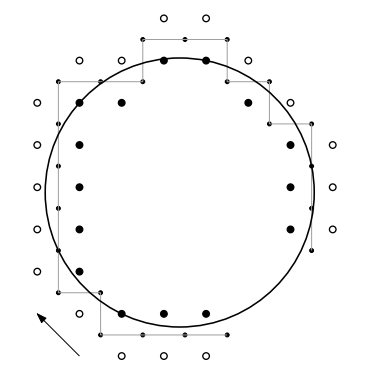
\includegraphics[height=6cm]{images/Notions/DCA}
    \end{center}}
    \caption[Arc de cercle digital.]{Arc de cercle digital (Figure~1.22 de \cite{Roussillon2009}).\label{fig:dca-figure}}
\end{figure}
%
\begin{definition}{\fakeTitle{Arcs de cercle digitaux}}
  \label{def:digital-circular-arc}
  %
  Soit $\Shape$ une forme convexe de $\R^2$, avec un champ de courbure continue.
  Le contour digital $\BdZ{\DigShape}$ pour $\DigShape = \DSh$ est un arc de
  cercle digital (\anglais{DCA}) si et seulement s'il existe un cercle euclidien
  qui sépare les points intérieurs à $\BdZ{\DigShape}$ des points digitaux extérieurs de
  $\BdZ{\DigShape}$ (voir \RefFigure{fig:dca-figure}).
  %
  \\
  %
  Un arc de cercle digital est maximal (\anglais{\MDCA}) si et seulement s'il ne
  peut être étendu dans aucune direction.
  %
\end{definition}
%
\section{Estimateurs digitaux d'aire, de volume, de moments, de positionnement de surface}
%
\subsection{Aire et volume digitaux}
%
\subsubsection{Aire et volume en comptant les points digitaux}
\label{sec:AreaByCounting}
%
Une façon simple de calculer l'aire ou le volume d'une forme digitale consiste à
compter le nombre de points digitaux appartenant à la forme. Plus formellement,
pour tout sous-ensemble $\DigShape \subset \Z^2$, l'estimateur digital d'aire au pas
de discrétisation $h$ est défini par :
%
\begin{equation}
  \AreaC(\DigShape, h) \EqDef h^2 \MCard(\DigShape)
\end{equation}
%
En dimension $3$, nous noterons l'estimateur digital de volume au pas de
discrétisation $h$ :
%
\begin{equation}
  \VolC(\DigShape, h) \EqDef h^3 \MCard(\DigShape)
\end{equation}
%
Maintenant, si ce sous-ensemble digital $\DigShape$ provient de la discrétisation de
formes euclidiennes $\Shape$, nous voulons que l'estimation du volume devienne
meilleure lorsque le pas de discrétisation $h$ se raffine (voir
\RefSection{sec:notion:multigridconvergence}). Il est connu depuis
\nauthor{Gauss} et \nauthor{Dirichlet} que cette façon d'estimer l'aire donne
des résultats de convergence asymptotique sur les formes $\Shape$ convexes
finies de $\R^2$ :
%
\begin{equation}
  \label{eq:AreaByCountingConv}
  \AreaC(\DigF{\Shape}{h},h) = \Area(\Shape) + O(h^\beta),
\end{equation}
%
avec $\beta = 1$ dans le cas général \cite{Klette2000}, et peut être optimisé à
$\beta = \frac{15}{11} - \epsilon$ avec $\epsilon > 0$ (arbitrairement petit)
lorsque le bord de l'objet est $C^3$ à courbure non nulle \cite{Huxley1990}.
De mêmes résultats ont été proposés en 3D :
%
\begin{equation}
  \label{eq:VolumeByCountingConv}
  \VolC(\DigF{\Shape}{h},h) = \Vol(\Shape) + O(h^\gamma),
\end{equation}
%
avec $\gamma = 1$ dans le cas général \cite{Kratzel1988}, et peut être amélioré à
$\gamma=\frac{243}{158}$ lorsque le bord est lisse \cite{Guo2010}.
%
En dimension 2, les objets non convexes suivent les mêmes règles tant que
$\Shape$ peut être exprimé comme une somme ou une différence de régions convexes
bornées par des courbes fermées simples \cite{Huxley1996}. Ces résultats
précédents restent valides chaque fois que le bord de la forme peut être
décomposé en nombre fini de morceaux convexes (ou convexe $C^3$ à courbure non
nulle pour les bornes améliorées).
%
\subsection{Moments géométriques digitaux}
%
Le concept mathématique des moments a beaucoup été étudié depuis plusieurs
années et trouve son champ d'application sans cesse augmenté, allant des
statistiques et mécaniques (\anglais{General moment theory}) \cite{} à la
reconnaissance de formes (\cauthors{Trier}{Trier1996} pour un survey sur la
reconnaissance de caractères, \cite{}) et la reconstruction d'objets \cite{Ghorbel2005}.
La première utilisation des moments en analyse d'images remonte à 1962 par
\cauthor{Hu}{Hu1962} pour la reconnaissance de caractères.
%
Les moments ont l'avantage d'être indépendant à l'échelle, la position et
l'orientation, en faisant un outil invariant robuste \cite{}. Nous allons tout
d'abord définir ce que sont les moments et leurs caractéristiques, pour ensuite
nous intéresser à les estimer sur des données digitales.
%
\todoJeremy{Le papier Reconstructing With Geometric Moments \cite{Ghorbel2005} est pas mal niveau intro}
%
\subsubsection{Définition et propriétés des moments géométriques}%
\label{sec:definitions-moments}
%
Une définition générale du moment géométrique (ou moment cartésien) $\Mom{p_1
\cdots p_d}$ d'ordre $p_1 \cdots p_d$ (aussi appelé le $p_1 \cdots p_d$-moment)
de $\Shape$ (de $\R^d$) peut être donnée comme :
%
\begin{equation}
  \Mom{p_1 \cdots p_d}(\Shape) \EqDef \idotsint_{\Shape} x_1^{p_1} \cdots x_d^{p_d} f(x_1 \cdots x_d) dx_1 \ldots dx_d.
\end{equation}
%
\paragraph{Moment d'ordre zéro : aire / volume}
%
Il apparaît alors que le $0\cdots0$-moment correspond à l'aire en 2D ou au
volume en 3D de $\Shape$ :
%
\begin{equation}
  \Mom{0 \cdots 0}(\Shape) \EqDef \idotsint_{\Shape} f(x_1 \cdots x_d) dx_1 \ldots dx_d.
\end{equation}
%
\paragraph{Moments du premier ordre : barycentre}
%
Les $d$ moments du premier ordre ($\Mom{1 0 \cdots 0}(\Shape)$, $\Mom{0 1 0
\cdots 0}(\Shape)$, $\cdots$, $\Mom{0 \cdots 0 1}(\Shape)$) sont généralement
utilisés pour déterminer le barycentre de la forme à analyser. Les coordonnées
du barycentre $(\overline{x_1}, \cdots, \overline{x_p})$ sont :
%
\begin{equation}
  \overline{x_1} = \frac{\Mom{1 0 \cdots 0}(\Shape)}{\Mom{0 \cdots 0}(\Shape)}, \cdots, \overline{x_p} = \frac{\Mom{0 \cdots 0 1}(\Shape)}{\Mom{0 \cdots 0}(\Shape)}.
\end{equation}
%
\paragraph{Moments du second ordre}
%
Les moments du second ordre $\Mom{p_1 \cdots p_d}(\Shape)$ avec $p_1 + \cdots +
p_2 = 2$ sont connus comme les moments d'inertie, caractérisant la géométrie des
masses de la forme. En 2D, nous en dénombrons 3 : $\Mom{2 0}(\Shape)$, $\Mom{1
1}(\Shape)$ et $\Mom{0 2}(\Shape)$, en 3D il en existe 6 :  $\Mom{2 0
0}(\Shape)$, $\Mom{0 2 0}(\Shape)$, $\Mom{0 0 2}(\Shape)$, $\Mom{1 1
0}(\Shape)$, $\Mom{0 1 0}(\Shape)$ et $\Mom{1 0 1}(\Shape)$
%
\subsubsection{Moments en comptant les points digitaux}
\label{sec:MomentsByCounting}
%
Comme pour l'aire ou le volume précédemment, il est très simple de calculer les
moments sur des données digitales. En effet, il suffit de sommer les valeurs des
points digitaux de la forme et de remettre à l'échelle suivant le pas de
discrétisation $h$. Plus formellement, pour tout sous-ensemble $\DigShape$ de
$\Z^d$, le $p_1 \cdots p_d$-moment digital de $\DigShape$ au pas de
discrétisation $h$ est défini par :
%
\begin{equation}
  \DMom{p_1 \cdots p_d}{h}(\DigShape) \EqDef h^{d + p_1 + \cdots + p_d} \sum_{(z_1,\ldots,z_d) \in \DigShape} z_1^{p_1} \cdots z_d^{p_d} f(z_1^{p_1} \cdots z_d^{p_d}).
\end{equation}
%
Il est à noter que $f(z_1 \cdots z_d)$ est tout le temps égal à $1$ lorsque
$(z_1,\ldots,z_d) \in \DigShape$, $0$ sinon, nous pouvons alors l'enlever de
l'équation :
%
\begin{equation} \label{eq:MomentsByCounting-def}
%
  \DMom{p_1 \cdots p_d}{h}(\DigShape) \EqDef h^{d + p_1 + \cdots + p_d} \sum_{(z_1,\ldots,z_d) \in \DigShape} z_1^{p_1} \cdots z_d^{p_d}.
%
\end{equation}
%
Ainsi, le $0$-moment digital de $\DigShape$ correspond au volume digital de
$\DigShape$, \cad $\AreaC(\DigShape,h)$ lorsque $d = 2$ et $\VolC(\DigShape,h)$
lorsque $d \geq 3$.
%
Nous souhaitons alors borner l'erreur entre les moments de $\Shape$ et
l'estimation des moments digitaux de la discrétisation de $\Shape$ comme
fonction du pas de discrétisation $h$. \cauthors{Klette}{Klette2000} ont
démontré la convergence de cet estimation des moments avec une vitesse de
convergence dépendante de l'ordre du moment $\sigma = p_1 + \cdots + p_d$ :
%
\begin{equation} \label{eq:MomentsByCounting-conv}
%
  \DMom{p_1 \cdots p_d}{h}(\DigF{\Shape}{h},h) = \Mom{p_1 \cdots p_d}(\Shape) + O(h^{\mu_{\sigma}}).
%
\end{equation}
%
avec $\mu_{\sigma} \ge 1$ dans le cas général (\todoJeremy{expliciter}). Cette
borne peut être améliorer lorsque la courbure gaussienne n'est pas nulle :
\cauthors{Krätzel}{Kratzel1991} obtiennent $\mu_0=\frac{38}{25}-\epsilon$ et
\cauthors{Müller}{Muller1999} obtiennent $\mu_0 = \frac{66}{43}-\epsilon$.
\todoInlineJeremy{A verifier}
%
\section{Enveloppes convexes}
%
